%%%%%%%%%%%%%%%%%%%%%%%%%%%%%%%%%%%%%%%%%%%%%%%%%%%%%%%%%%%%%%%%%%%%%%%%%%
% Bridge voltages and inductor current of the DAB, d > 1 (Exercise 08, Task 3)
%%%%%%%%%%%%%%%%%%%%%%%%%%%%%%%%%%%%%%%%%%%%%%%%%%%%%%%%%%%%%%%%%%%%%%%%%%

\begin{figure}[htb]
	\begin{center}
		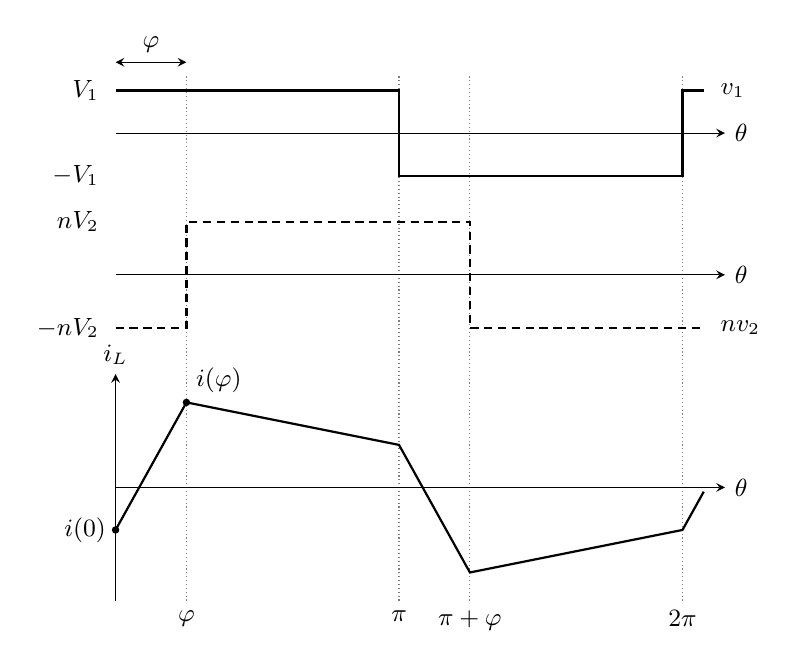
\begin{tikzpicture}[scale=0.9, >=stealth, every node/.style={font=\small}]
			% time marks
			\foreach \x/\l in {1/\varphi, 4/\pi, 5/\pi+\varphi, 8/2\pi}{
					\draw[densely dotted, gray] (\x,5.8) -- (\x,-1.6);
					\node[anchor=north] at (\x,-1.6) {$\l$};
				}
			\draw[<->] (0,6.0) -- (1,6.0) node[midway, above]{$\varphi$};
			% v1
			\draw[->] (0,5.0) -- (8.6,5.0) node[right]{$\theta$};
			\draw[thick] (0,5.6) -- (4,5.6) -- (4,4.4) -- (8,4.4) -- (8,5.6) -- (8.3,5.6);
			\node[anchor=east] at (-0.1,5.6) {$V_1$};
			\node[anchor=east] at (-0.1,4.4) {$-V_1$};
			\node[anchor=west] at (8.4,5.6) {$v_1$};
			% n v2
			\draw[->] (0,3.0) -- (8.6,3.0) node[right]{$\theta$};
			\draw[thick, densely dashed] (0,2.25) -- (1,2.25) -- (1,3.75) -- (5,3.75) -- (5,2.25) -- (8.3,2.25);
			\node[anchor=east] at (-0.1,3.75) {$nV_2$};
			\node[anchor=east] at (-0.1,2.25) {$-nV_2$};
			\node[anchor=west] at (8.4,2.25) {$nv_2$};
			% iL
			\draw[->] (0,0) -- (8.6,0) node[right]{$\theta$};
			\draw[->] (0,-1.6) -- (0,1.6) node[above]{$i_L$};
			\draw[thick] (0,-0.6) -- (1,1.2) -- (4,0.6) -- (5,-1.2) -- (8,-0.6) -- (8.3,-0.06);
			\fill (0,-0.6) circle (1.5pt) node[anchor=east]{$i(0)$};
			\fill (1,1.2) circle (1.5pt) node[anchor=south west]{$i(\varphi)$};
		\end{tikzpicture}
	\end{center}
	\caption{Bridge voltages and inductor current of the DAB with single phase shift for $d=nV_2/V_1>1$ (not to scale). The primary bridge switches at $\theta=0$, the secondary bridge at $\theta=\varphi$.}
	\label{fig:ex08_dab}
\end{figure}
